\section{Análise de opções tecnológicas}

Nesta seção está apresentada a análise das opções tecnológicas plausíveis para o atendimento dos requisitos. As alternativas pesquisadas e as escolhidas para cada parte do projeto estão explicitadas a seguir.

\subsection{Estação base}

As alternativas pesquisadas para a estação base estão apresentadas nesta subseção.

\subsubsection{Biblioteca para desenhos 2D}
\label{subsec:alternativas_desenho}

Tendo em vista que um dos requisitos é a geração de um mapa em duas dimensões na estação base, deve-se escolher uma biblioteca que permita realizar o desenho de formas geométricas em 2D (via código-fonte) e que possa ser integrada facilmente à interface gráfica. Ela deve também possuir meios simples de obter informações do mouse e teclado, para interatividade com o usuário. 

Uma biblioteca interessante disponível em Java que possui o recurso de produzir desenhos dinâmicos com integração a interfaces gráficas é o Processing \cite{processing}, de código livre. Essa biblioteca foi a principal encontrada que seria capaz de satisfazer as necessidades de desenho do mapa 2D de forma simples. Por possuir inúmeras funções de desenho em alto nível, o trabalho de renderização dos gráficos seria consideravelmente simplificado. Além disso, na biblioteca existem recursos que permitem o recebimento de informações de posicionamento do mouse e de comandos do teclado. Por ser constituído basicamente de um \textit{Applet} Java, o Processing pode facilmente ser integrado a componentes do Swing -- biblioteca de interface gráfica (GUI) do Java.


Outra biblioteca para a confecção de desenhos em 2D é o Cairo \cite{cairo}, que é \textit{open-source}, disponível nas linguagens C e C++. Ele possui recursos em alto nível para renderização de formas e interação com o usuário, assim como o Processing. Nos aspectos gerais as duas ferramentas são muito semelhantes. A integração do Cairo com a interface gráfica, porém, é dependente na biblioteca externa de GUI utilizada.

Um aspecto importante a notar é que ambas as bibliotecas foram desenvolvidas e otimizadas para terem bom desempenho em máquinas atuais -- o que é desejável tendo em vista os requisitos. Na Tabela \ref{tab:alternativas_desenho} está presente uma comparação entre as duas bibliotecas.


\begin{table}[h]
  \caption{Comparação entre Bibliotecas para desenhos 2D.}
  \centering
  \begin{tabular}{p{6cm}|p{4cm}p{4cm}}
    \toprule
    \textbf{Característica} & \textbf{Cairo} & \textbf{Processing} \\
    \midrule
    Linguagem de programação & C e C++ & Java \\
    \hline
    Integração com interface gráfica & Sim (depende da biblioteca de GUI utilizada) & Sim (com a biblioteca Swing do Java) \\
    \hline
    Ferramentas de interação com o usuário & Sim & Sim \\
    \bottomrule
  \end{tabular}
  \label{tab:alternativas_desenho}
\end{table}

\textbf{Escolha da equipe:} O Processing foi adotado como solução para desenhos 2D. Deve-se ressaltar que a escolha da biblioteca de desenhos foi feita em conjunto com a escolha de linguagem de programação, tendo em vista a interdependência de ambas. Em razão dos motivos apresentados na próxima subseção -- que se constituem de principal argumento para a escolha do Processing -- o Java foi adotado. Um ponto interessante do Procesing é a simplicidade de integração a interfaces gráficas (Swing) do Java.

\subsubsection{Linguagem de programação}

Na etapa de avaliação das opções tecnológicas, a escolha de uma boa linguagem de programação que atenda aos requisitos é fundamental. Abaixo está presente uma lista dos aspectos desejáveis da linguagem a ser utilizada neste projeto:

\begin{itemize}
  \item Deve ser multiplataforma (ao menos compatível com Linux e Windows sem muitas modificações);
  \item Deve possuir orientação a objetos;
  \item Deve possuir recursos multiplataforma e de código livre para o desenvolvimento de interfaces gráficas;
  \item Deve ter a disponibilidade de ferramentas de código livre e multiplataforma para a criação \textit{visual} da interface gráfica, dessa forma agilizando o processo de desenvolvimento;
  \item Deve possuir recursos, integrados ou em bibliotecas externas de código livre, para o desenvolvimento de desenhos dinâmicos (para a geração do mapa 2D). Os desenhos devem ser facilmente integráveis à interface gráfica.
\end{itemize}


Abaixo está presente uma descrição de duas linguagens, o C++ e Java, atualmente utilizadas em inúmeras aplicações, e que são potenciais alternativas ao projeto -- tendo em vista a experiência e conhecimento dos integrantes a respeito de ambas. A Tabela \ref{tab:alternativas_linguagens} sumariza os recursos de cada uma.

\textbf{Java}

O Java \cite{java} é uma linguagem concebida de início como sendo orientada a objetos. A maneira com que é feita a compilação e execução do código permite que, muito facilmente, programas sejam rodados em diferentes plataformas (Linux, Windows, Mac, entre outros). O processo de compilação do código gera os chamados \textit{bytecodes}, que são instruções a serem interpretadas pela \textit{Java Virtual Machine} (JVM). A grande vantagem é que o JVM possui disponibilidade multiplataforma, e a manutenção dele pelos desenvolvedores é frequente.

Há disponibilidade, na API do Java, da biblioteca Swing -- que contém recursos completos para a criação de interfaces gráficas (GUI) interativas. Existem ferramentas visuais de código aberto que consideravelmente agilizam o processo de desenvolvimento de interfaces Swing, entre elas o NetBeans \cite{netbeans} e o Eclipse \cite{eclipse}, através de plugins ou extensões. 

Para o preenchimento do requisito de confecção de desenhos em 2D com integração à interface gráfica, a biblioteca do Processing (explicada anteriormente na Subseção \ref{subsec:alternativas_desenho}) está disponível nessa linguagem.


\textbf{C++}

O C++ é uma linguagem orientada a objetos, que foi desenvolvida a partir da linguagem C. A compilação de código no C++ deve ser feita especificamente para cada plataforma em que um programa desenvolvido for utilizado. De uma perspectiva prática, certas seções de código frequentemente necessitam de adaptações manuais para cada plataforma e sistema operacional, o que gera retrabalho e gastos de tempo adicionais. 

Recursos para desenvolvimento visual de interfaces gráficas estão disponíveis através de bibliotecas e ferramentas externas. O C++ não possui recursos de interface gráfica na própria API e, portanto, deve-se notar que este é um aspecto complicador ao portar programas entre diferentes sistemas. 

Para a confecção de desenhos 2D e incorporação dos mesmos à interface gráfica, a biblioteca Cairo (explicada anteriormente na Subseção \ref{subsec:alternativas_desenho}) pode ser utilizada com essa linguagem. A possibilidade de haver integração com a interface, porém, é dependente da biblioteca de GUI utilizada.


\begin{table}[h]
  \caption{Comparação entre linguagens de programação.}
  \centering
  \begin{tabular}{p{6cm}|p{4cm}p{4cm}}
    \toprule
    \textbf{Característica} & \textbf{C++} & \textbf{Java} \\
    \hline
    Multiplataforma (Linux e Windows) & Sim (com adaptação) & Sim (sem adaptação) \\
    \hline
    Orientação a objetos & Sim & Sim \\
    \hline
    Recursos multi-plataforma e \textit{open-source} para desenvolvimento de interface gráfica (GUI) & Sim (com bibliotecas externas) & Sim (integrado à API da linguagem) \\
    \hline
    Ferramentas \textit{open-source} e multiplataforma para criação visual de interface gráfica & Sim (ferramentas externas) & Sim (ferramentas externas) \\
    \hline
    Recursos \textit{open-source} para desenvolvimento de desenhos dinâmicos, facilmente integráveis à interface gráfica & Sim (biblitoeca externa, integração à interface gráfica dependente da GUI utilizada) & Sim (biblioteca externa) \\
    \bottomrule
  \end{tabular}
  \label{tab:alternativas_linguagens}
\end{table}

\textbf{Escolha da equipe:} O Java foi a linguagem escolhida para o desenvolvimento do \textit{software} da estação base, uma vez que preenche satisfatoriamente os requisitos do projeto. Ressalta-se novamente que a escolha do Java foi feita em conjunto com a escolha da biblioteca do Processing. Notavelmente, no Java há a facilidade em portar, sem adaptações consideráveis na maioria dos casos, programas para diferentes plataformas -- processo este que é mais complexo no C++.  Com relação ao quesito de desempenho em computadores atuais, a linguagem escolhida é satisfatória, visto que há manutenção constante da implementação das bibliotecas e da máquina virtual do Java pelos desenvolvedores -- que buscam, entre outros aspectos, otimizar a linguagem para as tecnologias disponíveis atualmente.

\subsubsection{Sistema operacional}

Estando escolhida a linguagem de programação, o próximo passo é escolher um sistema operacional que seja compatível com ela e que satisfaça os requisitos da seção \ref{subsec:req_estacao-base}. Os aspectos desejáveis, portanto, são:

\begin{itemize}
  \item Deve ser compatível com o Java;
  \item Deve ser compatível com ferramentas de desenvolvimento \textit{visual} de interface gráfica;
  \item Deve ser gratuito e de código aberto.
\end{itemize}

A Tabela \ref{tab:alternativas_SO} apresenta uma comparação entre dois sistemas operacionais, Linux e Windows -- sobre os quais a equipe tem considerável experiência e possibilidade de uso nos próprios computadores pessoais.

\begin{table}[h]
  \caption{Comparação entre sistemas operacionais.}
  \centering
  \begin{tabular}{p{6cm}|p{2cm}p{2cm}}
    \toprule
    \textbf{Característica} & \textbf{Linux} & \textbf{Windows} \\
    \hline
    Compatível com Java & Sim & Sim \\
    \hline
    Compatível com ferramentas visuais de desenvolvimento & Sim & Sim \\
    \hline
    Gratuito e de código aberto & Sim & Não \\
    \bottomrule
  \end{tabular}
  \label{tab:alternativas_SO}
\end{table}

\textbf{Escolha da equipe:} Ambos os sistemas comparados são compatíveis com o Java e com ferramentas visuais de desenvolvimento de interface gráfica (NetBeans e Eclipse). Porém, o Linux é o único gratuito e de código aberto, e portanto foi o sistema operacional escolhido para o desenvolvimento do projeto da estação base.



\subsection{Sistema de comunicação}

Como foi explicitado nos requisitos, o sistema de comunicação ter as seguintes características:

\begin{itemize}
  \item Alcance de, no mínimo, 20 metros sem fios;
  \item Velocidade suficiente para, simultaneamente, o envio de comandos de movimentação ao robô, recebimento de dados de leituras de sensores e recebimento de imagens da câmera;
  \item Fluxo de dados bidirecional (\textit{full-duplex});
  \item Utilização simples do protocolo TCP.
\end{itemize}

Para o cálculo da taxa de transmissão mínima necessária, faz-se uma estimativa inicial. Prevê-se que o envio de imagens da câmera é o que mais utilizará os recursos da conexão. Supondo serem usadas a máxima qualidade e taxa de amostragem suportadas por uma câmera VGA comum (resolução 640x480, RGB 24 bits, 30 FPS), além de uso de compressão JPEG com 90\% de qualidade, haverá uso de aproximadamente 2,4 MB/s ou 19,2 MBits/s \cite{webcam_resolution}. 

O envio de comandos ao robô, supondo que cada comando tenha 2 KB e hajam 10 comandos por segundo (estimativa exaregada), gastará em torno de 160 KBits/s. O recebimento de informações do robô e leituras dos sensores, supondo que cada pacote tenha 2 KB (com exagero) e haja recebimento de 10 pacotes por segundo, utilizará 160 KBits/s na banda da conexão. Portanto, o valor mínimo desejável da taxa de transferência é de 19,2 + 0,16 + 0,16 = 19,52 MBits/s.

Na Tabela \ref{tab:alternativas_comunicacao} está presente uma comparação entre diferentes tecnologias de comunicação sem fios, que potencialmente podem satisfazer às necessidades do projeto. 


\begin{table}[h]
  \caption{Comparação entre tecnologias de comunicação sem fios.}
  \centering
  \begin{tabular}{p{4.5cm}|p{3cm}p{4cm}p{2cm}}
    \toprule
    \textbf{Característica} & \textbf{802.11g (Wi-Fi)} & \multicolumn{1}{l}{\textbf{Rádio Frequência (RF)}} & \textbf{Bluetooth}  \\
    \hline
    Distância máxima de alcance & 50-100 metros  & 30-100 metros & 10 metros \\
    \hline
    Velocidade de transmissão máxima & 54 Mbits/s & 2 Mbits/s & 1 Mbits/s \\
    \hline
    Fluxo de dados \textit{full-duplex} & Sim & Sim & Sim \\
    \hline
    Possibilidade e simplicidade de uso de TCP & Sim & Não & Não \\
    \bottomrule
  \end{tabular}
  \label{tab:alternativas_comunicacao}
\end{table}

\textbf{Escolha da equipe:} O Wi-Fi é o recurso mais atrativo em todos os aspectos que foram comparados, preenchendo satisfatoriamente os requisitos do sistema de comunicação. Sua velocidade e alcance são suficientes para satisfazer as necessidades do projeto, e o fluxo de dados pode ser \textit{full-duplex}. Notavelmente, o Wi-Fi é o único sistema comparado que oferece a possibilidade (com simplicidade) de uso do protocolo TCP -- o que é um requisito importante para o desenvolvimento ágil e satisfatório do projeto.

É importante ressaltar que uma conexão Wi-Fi 802.11g dedicada será utilizada para a comunicação entre o robô e a estação base, de modo que a velocidade de conexão possa ser utilizada com maior eficiência sem interferências de outros utilizadores.


\subsection{Sistema embarcado}
\label{subsec:opcoes_sist-embarcado}
Nesta seção serão apresentadas as alternativas pesquisadas para o sistema embarcado, levando-se em conta os requisitos da Seção \ref{subsec:req_sistema-embarcado}.

\subsubsection{Imagens instantâneas do ambiente}

Para a obtenção de imagens do ambiente onde o robô se encontra, optou-se por utilizar uma \textit{webcam} USB conectada à placa TS-7260 já presente no robô. Essa placa possuirá o \textit{hardware} de comunicação Wi-Fi do robô, e deve-se relembrar que um único canal sem fios será utilizado (como explicitado nos requisitos). Mostra-se adequada, portanto, a utilização de uma câmera que possa ser conectada por USB à placa, de modo que as imagens possam ser transmitidas por esse canal Wi-Fi. Abaixo estão listadas as características desejáveis da \textit{webcam}:

\begin{itemize}
  \item Possuir conexão USB 2.0;
  \item Ser compatível com Linux;
  \item Ser capaz de, no mínimo, produzir imagens em resolução VGA (640x480), RGB 24 bits a 30 fps, para que a visualização possa ser feita com qualidade satisfatória.
\end{itemize}

A compatibilidade com o Linux pode ser garantida com a escolha de uma \textit{webcam} em conformidade com o padrão UVC (\textit{USB Video Class}) e compatível com o \textit{driver} Video4Linux 2 (V4L2), presente nos \textit{kernels} do Linux a partir da versão 2.5. Uma lista de dispositivos que seguem esse padrão está disponível em \cite{uvc-linux}. Três câmeras de custo baixo e com disponibilidade no Brasil foram selecionadas a partir da lista, como apresentado na Tabela \ref{tab:alternativas_camera}.


\begin{table}[h]
  \caption{Comparação entre \textit{webcams} USB.}
  \centering
  \begin{tabular}{p{5cm}|p{3.3cm}p{3cm}p{2.5cm}}
    \toprule
    \textbf{Característica} & \textbf{Genius FaceCam 2000} & \multicolumn{1}{l}{\textbf{Microsoft VX-500}} & \textbf{Genius iSlim 1300}  \\
    \hline
     Conexão USB 2.0 & Sim & Sim & Sim  \\
     \hline
     Compatível com Linux & Sim & Sim & Sim \\
     \hline
     Resolução máxima de vídeo & 1620X1200 & 640x480 & 1280X1024 \\
     \hline
     RGB 24 bits & Sim & Sim & Sim \\
     \hline 
     Taxa de amostragem & 30 fps & 30 fps & 30 fps \\
     \hline
     Custo & R\$ 82,00 & R\$ 79,50 & R\$ 34,99 \\
    \bottomrule
  \end{tabular}
  \label{tab:alternativas_camera}
\end{table}

Percebe-se que as características técnicas de todas as três câmeras são satisfatórias para o preenchimento dos requisitos. Porém, há certas diferenças relacionadas a custo e resolução.

\textbf{Escolha da equipe:} A \textit{webcam} escolhida foi a Genius iSlim 1300, principalmente tendo em vista o seu custo muito reduzido em relação às outras. Além disso, possui resolução muito satisfatória. Em Curitiba, há disponibilidade desse modelo em pronta entrega.

\begin{figure}[H]
\centering
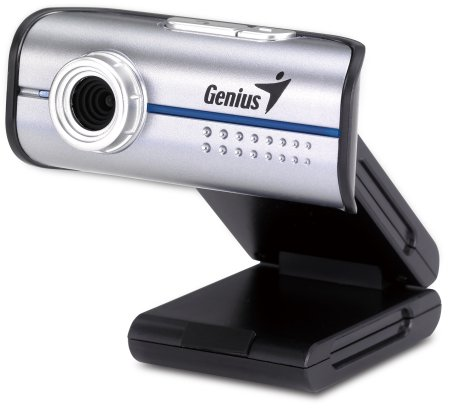
\includegraphics[width=0.4\textwidth]{./figuras/quali/genius-slim1300.jpg}
\caption{\textit{Webcam} Genius iSlim 1300.}
\fonte{\cite{genius-islim-1300}}
\label{fig:genius-islim-1300}
\end{figure}

\subsubsection{Movimentação do robô}

Uma vez que o sistema de movimentação do robô, incluindo motores, acionadores, drivers de potência e rodas já estão instalados no robô e atendem aos requisitos, não houve nova pesquisa sobre esses componentes. Um chassi de 40 cm de largura por 50 cm de comprimento, duas rodas de tração e uma roda guia estão presentes atualmente. As rodas de tração estão dispostas na parte posterior do robô, possuindo 20 cm de diâmetro e 4 cm de largura. O chassi está equipado com 2 motores Bosch FPG 12V, 2 baterias Unybatt 12V-7,2 Ampére-hora e duas pontes H L298 \cite{bellator_2012}. A disposição dos itens no robô pode ser vista na figura \ref{fig:disposicao_bellator_2012}.

\begin{figure}[H]
\centering
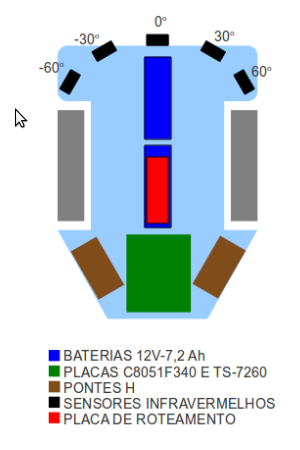
\includegraphics[width=0.4\textwidth]{./figuras/quali/disposicao-robo.png}
\caption{Disposição dos itens no robô}
\fonte{\cite{bellator_2012}}
\label{fig:disposicao_bellator_2012}
\end{figure}

\subsubsection{Odometria}

Para a obtenção da aceleração, velocidade e posição do robô, diversas tecnologias podem ser escolhidas. Abaixo serão descritas as principais opções:

\begin{itemize}
  \item \textbf{Encoder:} Ligado ao eixo da roda do robô, efetua a contagem das rotações realizadas por ela, permitindo assim calcular a distancia percorrida. Se dois encoders forem instalados, um em cada roda, a direção do movimento poderá ser obtida a partir de cálculos baseados na contagem de voltas de cada roda.
  \item \textbf{GPS:} Utiliza sinais de satélites para obter as coordenadas geográficas do robô. A direção e o sentido do movimento podem ser obtidos a partir da comparação das leituras atuais com as anteriores.
  \item 	\textbf{Acelerômetro:} Pode utilizar a tecnologia chamada MEMS para medir a aceleração do componente. A velocidade e deslocamento lineares podem ser obtidos por integração numérica da aceleração.
  \item 	\textbf{Giroscópio:} Pode utilizar a tecnologia chamada MEMS para medir a velocidade angular do componente. O ângulo de rotação pode ser obtido por integração numérica da velocidade angular.
  \item 	\textbf{Bússola:} Utiliza os campos magnéticos da terra para obter a orientação geográfica absoluta do robô.
\end{itemize}

Na Tabela \ref{tab:alternativas_tecnologias_odometria} está presente uma comparação entre as tecnologias apresentadas. 

\begin{table}[h]
  \caption{Comparação entre tecnologias para odometria.}
  \centering
  \begin{tabular}{p{3cm}|p{2.2cm}p{1.7cm}p{2.2cm}p{2.2cm}p{2.2cm}}
    \toprule
    \textbf{Característica} & \textbf{Encoder} & \textbf{GPS} & \textbf{Acelerômetro} & \textbf{Giroscópio} & \textbf{Bússola} \\
    \hline
    Sujeito a influencias externas & Deslizamentos & Não & Não & Não & Ruídos de campos magnéticos diversos \\
    \hline
    Ambiente de operação & Interno / Externo & Externo & Interno / Externo & Interno / Externo & Interno / Externo \\
    \hline
    Posicionamento & Relativo & Absoluto & Relativo & Relativo & Absoluto \\
    \hline
    Acumulo de erro para calculo da posição & Sim & Não & Sim (duas integrações) & Sim (uma integração) & Sim \\
    \bottomrule
  \end{tabular}
  \label{tab:alternativas_tecnologias_odometria}
\end{table}

Da Tabela \ref{tab:alternativas_tecnologias_odometria}, vê-se que \textit{encoders} estão sujeitos a erros causados por deslizamentos nas rodas, e que GPS apenas funciona em ambientes externos. A bússola pode ser influenciada por campos magnéticos diferentes do da terra -- como por exemplo o gerado pelos motores. O acelerômetro e o giroscópio por sua vez acumulam o erro de duas integrações e uma integração respectivamente\footnote{A aceleração linear e velocidade angular devem ser integradas numericamente duas vezes e uma vez respectivamente para cálculo da posição: Uma vez para determinação da velocidade linear; E outra vez para determinação do deslocamento e ângulo de rotação atuais.} para obtenção da posição.

\textbf{Escolha da equipe:} Os \textit{encoders} estão sujeito apenas aos erros de deslizamentos e acumulam menos erros na obtenção da posição do que os giroscópios e acelerômetros. Sendo assim eles foram a escolha como principal fonte de dados para odometria. O GPS não foi escolhido pois opera apenas em ambientes externos. A bússola por sua vez poderá sofrer influencias do campo magnético gerado pelos motores do robô. Como a utilização apenas dos \textit{encoders} pode levar a erros no posicionamento devido a deslizamentos, utilizaremos também um acelerômetro e um giroscópio como fonte de dados auxiliar para possibilitar o aumento da exatidão e confiabilidade dos dados obtidos dos \textit{encoders}. Caso discrepâncias consideráveis ocorram entre os dados obtidos pelos sensores, escorregamentos das rodas podem ser detectados e mitigados, atenuando dessa forma erros na determinação do posicionamento.

Por exemplo, em caso de escorregamento roda, um \textit{encoder} fornece uma medição de velocidade maior do que a que corresponde à realidade do movimento do robô. O acelerômetro e o giroscópio, por sua vez, não sofrem influências do escorregamento das rodas, e tenderão a fornecer uma medida mais próxima à realidade. Discrepâncias nas medições podem ser dessa forma detectadas, e procedimentos de atenuação de erros (como por exemplo, descarte de certas medidas dos \textit{encoders}) poderão ser executados no \textit{software} da estação base.

%Esses dados servirão como entrada para um filtro de Kalman Estendido que calculará o estado (aceleração, velocidade e posição) do robô para um dado instante de tempo \cite{kalman_made_easy}, \cite{handbook_of_robotics}.
%%NOTA (Stefan):
%% Acho melhor não colocarmos essa questão do filtro de Kalman estendido agora, pois podemos ter sérios problemas para implementar isso depois. 
%% O filtro de Kalman que eu havia implementado foi uma versão simplificada, que recebe dados de apenas um sensor.

Os \textit{encoders} que serão utilizados (HEDS-9700) já se encontram acoplados ao robô, logo os motivos para a escolha do modelo não serão analisados.
Quanto ao acelerômetro e giroscópio, está apresentado a seguir, na Tabela \ref{tab:alternativas_componentes_odometria}, um comparativo entre as opções de menor custo disponíveis no mercado. Na Tabela estão listados apenas os modelos que possuem placas de desenvolvimento, pois acelerômetros e giroscópios geralmente são vendidos em encapsulamento LGA ou BGA (que são de difícil soldagem).

\begin{table}[h]
  \caption{Comparação entre acelerômetros/giroscópios para odometria.}
  \centering
  \begin{tabular}{p{2.4cm}|p{3cm}p{0.8cm}p{1.4cm}p{1.9cm}p{1.7cm}p{1.3cm}}
    \toprule
    \textbf{Modelo} & \textbf{Fabricante} & \textbf{Acel.} & \textbf{Giro.} & \textbf{Faixa} & \textbf{Interface} & \textbf{Preço} \\
    \hline
    STEVAL-MKI009V1	& STMicroeletronics & 3x	& - & $ \pm 2g$ ou $\pm 6g $ & I2C / SPI & \$23.94 \\
    \hline
	ATAVRSBIN1 & Atmel & 1x & - & - & I2c & \$26.25 \\
	\hline
	KIT3803 MMA7660FC & Freescale & 3x & - & $ \pm 1.5g $ & I2C & 	\$35.0 \\
	\hline
	ATAVRSBIN1 & Atmel & - & 1x & & I2C & \$26.25 \\
	\hline
	MPU-6050	 & IvenSense & 3x & 3x & $ \pm 2g$ ou $\pm 4g $; $ \pm 250 ^{o}/seg$ ou $ \pm 500 ^{o}/seg $ & I2C & \$8.78 \\
    \hline
	MKI086V1	 & STMicroeletronics & - & 1x & $ \pm 30^{o}/seg $ & Analog & \$31.50 \\
	\hline
	STEVAL-MKI094V1 & STMicroeletronics & - & 3x & $ \pm 400^{o}/seg $ & Analog & \$31.50 \\
	\hline
	ATAVRSBIN1 & Atmel & 1x & 1x & & I2C & \$26.25 \\
	\hline
	DM240316	 & Zena & 3x & 3x & 	& RF & \$99.99 \\
    \bottomrule
  \end{tabular}
  \label{tab:alternativas_componentes_odometria}
\end{table}

\textbf{MPU-6050}

Com base na Tabela \ref{tab:alternativas_componentes_odometria}, o modelo MPU-6050 da IvenSense foi escolhido, principalmente devido ao seu baixo custo: \$8.78. Este modelo possui um acelerômetro e um giroscópio (ambos de 3 eixos), além entradas para uma bussola externa de 3 eixos, tudo integrado a um único chip \cite{mpu6050}. A faixa de operação para o acelerômetro é de $ \pm 2g$ ou $\pm 4g $ e para o giroscópio é de $ \pm 250~ ^{o}/seg $ ou $ \pm 500~ ^{o}/seg $. A sensibilidade do acelerômetro é de $ 16384~ LSB/g $ ou $ 8192~ LSB/g $. A sensibilidade do giroscópio é de $ 131~ LSB/ (^{o} / seg) $ ou $ 65.5~ LSB/ (^{o} / seg) $. A interface de comunicação do módulo suporta o protocolo I2C. O módulo contendo o chip MPU-6050 e alguns componentes necessários para seu funcionamento pode ser visto na figura \ref{fig:mpu6050}.

\begin{figure}[H]
\centering
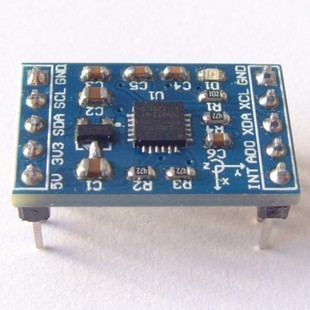
\includegraphics[width=0.4\textwidth]{./figuras/quali/mpu6050.JPG}
\caption{Placa de desenvolvimento contendo o chip MPU-6050}
\fonte{\cite{mpu6050}}
\label{fig:mpu6050}
\end{figure}

\textbf{Encoder Optico HEDS-9700}

Como foi explicitado anteriormente, os \textit{encoders} ópticos já existentes no robô serão utilizados. Ele está equipado com duas unidades do modelo HEDS-9700.
Quanto ao funcionamento, este modelo gera em sua saída uma onda quadrada à medida em que as rodas são rotacionadas, sendo 1800 pulsos gerados em uma rotação completa. A forma de onda da saída do \textit{encoder} pode ser vista na Figura \ref{fig:heds9700}. Pode-se ver na Figura que o \textit{encoder} possui duas saídas, A e B com defasamento $\phi$ entre elas. O sentido de rotação pode ser determinado pela informação de qual sinal (A ou B) está mais adiantado em fase \cite{heds9700}. A leitura e contagem das rotações do encoder serão feitas conforme foi desenvolvido no projeto anterior (descrito em \citeonline{bellator_2012}).

\begin{figure}[H]
\centering
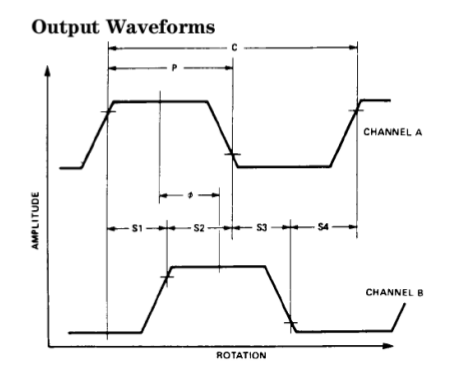
\includegraphics[width=0.6\textwidth]{./figuras/quali/heds9700.png}
\caption{Forma de onda na saída do encoder}
\fonte{\cite{heds9700}}
\label{fig:heds9700}
\end{figure}

\subsubsection{Detecção de obstáculos}

\textbf{Sensor de proximidade Infra Vermelho IR 2Y0A02F98}

A detecção de obstáculos, que é um requisito para o projeto robô, será feita pelos sensores de Infra Vermelho já existentes nele. Estão presentes 5 unidades do modelo IR 2Y0A02F98 \cite{ir_sensor}. Uma característica interessante deste sensor é que ele sofre pouca influência das cores dos objetos, devido ao método de medição baseado em triangulação. Na figura \ref{fig:ir_sensor_response} pode-se verificar o fato. A linha tracejada é a resposta para reflexão em uma superfície cinza e a linha contínua é a resposta para reflexão em uma superfície branca.

\begin{figure}[H]
\centering
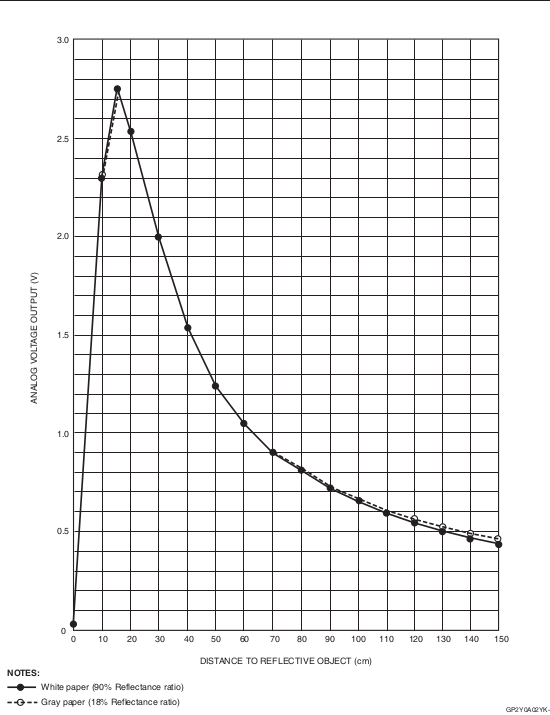
\includegraphics[width=1\textwidth]{./figuras/quali/ir-sensor-response.png}
\caption{Curva de resposta do sensor Infra Vermelho IR 2Y0A02F98}
\fonte{\cite{ir_sensor}}
\label{fig:ir_sensor_response}
\end{figure}

\subsubsection{Microcontrolador}

A interface entre sensores e atuadores (sistemas de acionamento dos motores) com a placa TS-7260 \footnote{Deve-se ressaltar que os atuadores (sistemas de acionamento dos motores) e a placa TS-7260 já existem no robô \cite{bellator_2012}.} será feita por um sistema microcontrolado. Este sistema deve possuir as interfaces adequadas para comunicação com todos os componentes. Na Tabela \ref{tab:requisitos_microcontrolador} estão listados os requisitos mandatórios para escolha do microcontrolador, e na Tabela \ref{tab:requisitos_desejaveis_microcontrolador} estão listados os requisitos desejáveis (porém não obrigatórios).

\begin{table}[h]
  \caption{Requisitos mandatórios para escolha do microcontrolador.}
  \centering
  \begin{tabular}{p{7cm}|p{8cm}}
    \toprule
    \textbf{Requisito} & \textbf{Justificativa} \\
    \hline
    Interface I2C & Comunicação com acelerômetro e giroscópio \\
    \hline
    Geração de PWM em 4 canais & Acionamento dos motores pelas pontes H \\
    \hline
    Interface Serial	 & Comunicação com a placa TS-7260 \\
    \hline
    Interrupções em 2 canais	 \\ (com capacidade de processamento de no minimo 2865 interrupções/segundo em cada canal \footnotemark ) & Leitura do valor dos \textit{encoders} \\
    \hline
    Conversor AD em 5 canais	 & Leitura dos sensores de IR \\
    \bottomrule
  \end{tabular}
  \label{tab:requisitos_microcontrolador}
\end{table}

%Texto do Footnote marcado na tabela anterior (\footnotemark).
\footnotetext{Valor calculado com base no tamanho das rodas, supondo velocidade máxima de deslocamento de $1m/s$.}

\begin{table}[h]
  \caption{Requisitos desejáveis para escolha do microcontrolador.}
  \centering
  \begin{tabular}{p{7cm}|p{8cm}}
    \toprule
    \textbf{Requisito desejável} & \textbf{Justificativa} \\
    \hline
    Desenvolvimento em plataforma livre	 & Diminuição do custo de softwares para desenvolvimento \\
    \hline
    2 Interfaces seriais ou JTAG & Utilização para \textit{debug} ou \textit{logs} \\
    \hline
    Solução integrada em um único chip & Redução do tamanho da placa e da quantidade de componentes, diminuindo assim o custo e melhorando a organização e disposição dos mesmos \\
    \bottomrule
  \end{tabular}
  \label{tab:requisitos_desejaveis_microcontrolador}
\end{table}

Na Tabela \ref{tab:alternativas_microcontrolador} estão listados diversos microcontroladores que foram pesquisadas para o projeto. Todos os modelos atendem aos requisitos da Tabela \ref{tab:requisitos_microcontrolador}.

\begin{table}[h]
\caption{Comparativo entre microcontroladores.}
\fonte{Dados obtidos de \cite{digikey}}
\centering
\begin{tabular}{l|rrrrrr}
\toprule
\textbf{uC} & \textbf{STM32F103C6T7A} & \textbf{PIC32MX320F128H} & \textbf{LPC2103} \\ \hline
Fabricante & STMicroelectronics & Microchip Technology & NXP Semiconductors \\ \hline
Arquitetura & ARM® Cortex™-M3 & MIPS32® M4K™ & ARM7 \\ \hline
Core & 32bits & 32-Bit & 16/32-Bit \\ \hline
Velocidade & 72MHz & 80MHz & 70MHz \\ \hline
MIPS & 90 & 124.8 & 63 \\ \hline
I2C & 1 & 2 & 2 \\ \hline
PWM & 12 & 5 & 14 \\ \hline
UART & 2 & 2 & 2 \\ \hline
Einterrupt & 16 & 5 & 13 \\ \hline
FLASH & 32k & 128k & 32k \\ \hline
RAM & 10k & 16k & 8k \\ \hline
Adc & 10x12b & 16x10b & 8x10b \\ \hline
JTAG & sim & sim & sim \\ \hline
Custo & \$6.27 & \$6.26 & \$6.16 \\
\toprule
\textbf{uC} & \textbf{MCF52210CAE66} & \textbf{AT32UC3C264C} & \textbf{SIM3C146} \\ \hline
Fabricante & Freescale Semiconductor & Atmel & Silicon Laboratories Inc \\ \hline
Arquitetura & Coldfire V2 & AVR & ARM® Cortex™-M3 \\ \hline
Core & 32-Bit & 32-Bit & 32-Bit \\ \hline
Velocidade & 66MHz & 66MHz & 80MHz \\ \hline
MIPS & 75.9 & 98.34 & 100 \\ \hline
I2C & 2 & 3 & 2 \\ \hline
PWM & 4 & 8 & 8 \\ \hline
UART & 3 & 1 & 2 \\ \hline
Einterrupt & 7 & 7 & 16 \\ \hline
FLASH & 64k & 64k & 64k \\ \hline
RAM & 16k & 16k & 16k \\ \hline
Adc & 8x12b & 11x12b & 28x12b \\ \hline
JTAG & sim & sim & SIM3C146-B-GQ \\ \hline
Custo & \$7.1 & \$9.14 & \$6.1 \\ \bottomrule
\end{tabular}
\label{tab:alternativas_microcontrolador}
\end{table}

\textbf{Escolha da equipe:} Dentre as opções listadas na Tabela \ref{tab:alternativas_microcontrolador}, o modelo LPC2103 foi escolhido. A escolha foi feita baseando-se principalmente no custo do microcontrolador. Nota-se, a primeira vista ao efetuar-se uma comparação com o SIM3C146, que essa última opção possui desempenho melhor e custo ligeiramente menor. Porém a escolha do LPC2103 justifica-se pela melhor documentação e mais ampla disponibilidade de recursos para o mesmo. A documentação fornecida pelo fabricante desse microcontrolador é mais completa e, pelo fato do modelo estar há mais tempo no mercado, a quantidade de informações e recursos disponíveis na \textit{internet} é maior.

\textbf{LPC2103}

O LPC2103 é um microcontrolador baseado na arquitetura ARM7TDMI-S da NXP \cite{lpc2103}. Este microcontrolador pode operar em até $ 70MHz $ executando a $ 63MIPS $. O Microcontrolador possui 2 interfaces I2C, 2 interfaces seriais, até 14 saídas de PWM, até 13 canais de interrupções externas, 8 canais de conversão para um conversor analógico digital de 10 bits, 32kbytes de memória FLASH para código e 8kbytes de memória RAM. Ele também suporta \textit{debug} via JTag por meio de um \textit{debugger} externo. O custo desse microcontrolador é de \$6.16 \cite{digikey}. O LPC2103 está disponível em encapsulamento LQFP com 48 pinos.

O microcontrolador escolhido pode também ser programado utilizando o protocolo ISP, por meio de ferramentas livres como o lpc21isp \cite{lpc21isp}. Para a geração do código hexadecimal utilizado pelo lpc21isp, basta efetuar a compilação de código em C utilizando o GCC \cite{gcc}.
Pode-se notar que o LPC2103, além de atender aos requisitos mandatórios da Tabela \ref{tab:requisitos_microcontrolador}, também atende aos requisitos desejáveis que foram expostos na Tabela \ref{tab:requisitos_desejaveis_microcontrolador}.

\subsubsection{Placa de circuito impresso}

A placa de circuito impresso será projetada utilizando ferramentas livres, como o gEDA \cite{geda} e PCB \cite{pcb}. Após o projeto da placa os arquivos \textit{Gerber} serão enviados à empresa Stick \cite{stick} para impressão. A soldagem dos componentes será realizada pela própria equipe.

Deve-se ressaltar que como, em geral, na soldagem de um \textit{chip} com encapsulamento LQFP há complexidade e riscos consideráveis (como por exemplo, queima do \textit{chip} ou da placa), a equipe pesquisou informações sobre \textit{kits} de desenvolvimento que tenham o LPC2103 já soldado na placa. Em Curitiba, existe a empresa eSysTech \cite{esystech} que fabrica tais \textit{kits}. Através de contatos da UTFPR, confirmou-se que na universidade há algumas unidades (fabricadas por essa empresa) que podem ser emprestadas à equipe para a realização do projeto, caso haja necessidade.
